\subsection{Sensors}\label{sec:sensors}
    \begin{figure}[H]
        \centering
        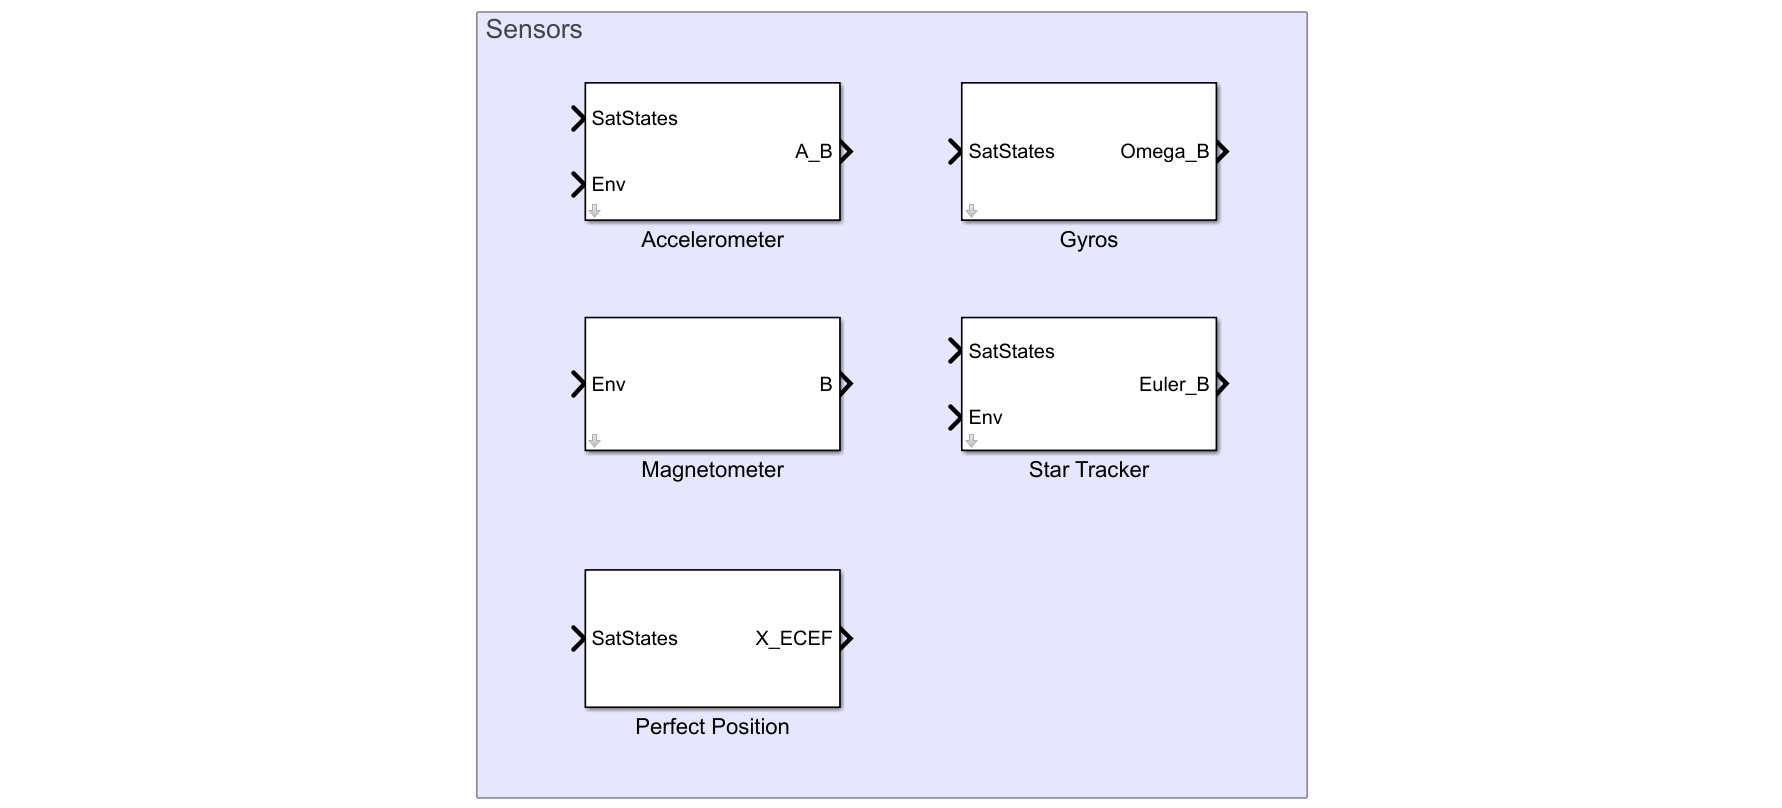
\includegraphics[width=0.7\textwidth]{2-toolbox/sensors.png}
        \caption{All Sensors blocks available in SCARS Parts Library}
        \label{fig:sensors}
    \end{figure}

    For precise orbit, or attitude, determination both sensors and mathematical models have to be used. Spacecraft sensors can be divided into two types, based on the nature of the performed measurement. One type, inertial sensors reflect the rate of change, therefore any other source of measurement is needed, for initial value acquisition and integration error correction. On the other side there are reference sensors, providing absolute measurements. Sensors of this type measure external parameters, such as Sun's position or Earth's magnetic field intensity, which when compared against mathematical or empirical models can bare the information about satellite's position or attitude. This division is visible in \ac{scars} models, as inertial sensors require input of satellite states, while reference sensors need input from environment model.

    It is important to mention, that it is possible to model sensors with various degrees of fidelity and different focus. For example, the influence of mechanical parameters on output signal of gyroscope is significant, resulting in a need for modeling it with transfer function describing its properties. On the other hand, in sensors such as star tracker the output is mostly processed in the software, therefore the focus is put on modeling the influence of spacecraft kinematics on the sensor, such as blinding the camera by the sun.

    \subsubsection{Ideal and Simple Sensor}
        Ideal Sensor is a Simulink subsystem block with unit gain inside, used for testing satellite behavior when sensor errors do not need to be taken into consideration.

        Simple Sensor is not a model of any specific type of sensor. It takes most common parameters used to transform generic ideal sensor into model which corresponds to real hardware, that is: sampling frequency, measurement range and most common sources of errors.

        % In the toolbox the following sources of gyroscope errors are modeled:
        % \begin{itemize}
        %     \item Bias offset:
        %     \item Scale factor: 
        %     \item \ac{arw}: A high frequency noise term that has a correlation time much shorter than the sample time. Can be defined as white noise component on the sensor output. Specified either in $\frac{deg}{\sqrt{h}}$ or, as a power spectral density, in $\frac{(deg/h)^2}{Hz}$. % cite this here: http://citeseerx.ist.psu.edu/viewdoc/download?doi=10.1.1.210.1133&rep=rep1&type=pdf
        %     \item Quantization Error: An error which is caused by the digital quantization of output signal, obtained when sampling analog input.
        %     \item ...
        % \end{itemize}

        % \dots\textit{description of implementation}\dots

    \subsubsection{GPS Receivers}
        The \ac{gps} is a \ac{gnss} owned adn operated by United States government. It allows determining position, velocity and time with data taken from at least four \ac{gps} satellites.

        Previously using \ac{gps} receivers in \ac{leo} was burdened with technical challenges, as off-the-shelf components were mostly designed for terrestrial operations, not encompassing for example for large variations in the received signal Doppler frequencies. Recently smaller \ac{gps} receivers became available, even for CubeSat use, such as \textit{Venus838FLPx GPS Receiver}\cite{gpsdatasheet}, allowing real time orbit determination using \ac{gps} navigation in smaller satellite projects.\cite{gomes2007real} When choosing a \ac{gps} receiver one must take several parameters into consideration: update rate, horizontal position accuracy, vertical position accuracy, velocity accuracy and failure rate.
        
        % \begin{itemize}
        %     \item Update rate
        %     \item Horizontal position accuracy
        %     \item Vertical position accuracy
        %     \item Velocity accuracy
        %     % \item Decay factor?
        %     \item Failure rate
        % \end{itemize}

        All listed parameters are set up in \ac{scars} \textit{GPS Receiver} part, but rather than designing a model from scratch, MATLAB's Navigation Toolbox function, \verb|gpsSensor()|, was nested inside a masked Simulink block. User can set all beforementioned parameters by editing \ac{gps} model's mask fields. Inputs of the model are satellite's true position and true velocity, and the outputs are position and velocity as computed by \ac{gps} receiver.


    \subsubsection{Accelerometers}
        \begin{figure}[H]
            \centering
            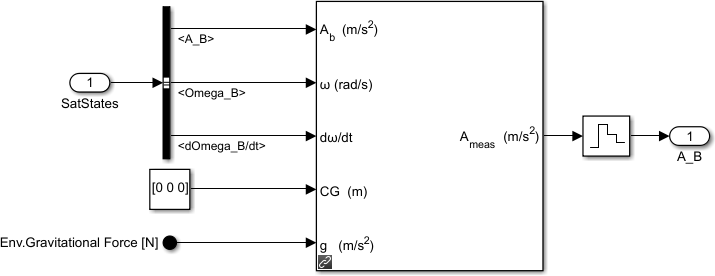
\includegraphics[width=1\textwidth]{2-toolbox/accelerometer.png}
            \caption{SCARS Accelerometer model}
            \label{fig:accelerometer}
        \end{figure}
        % accelerometer misalignment
        Accelerometers are force sensors, most often paired with gyroscopes as a part of \ac{imu} board. To find acceleration three sensors are located with their axes mutually orthogonal and the force external to the board is measured (with the exception of the gravitational force, as it likewise influences the proof mass of the sensor). These measurements are integrated once to obtain the velocity of the spacecraft with respect to the inertial space, or twice to calculate estimated position.

        Accelerometer model in \ac{scars} is based on Three-axis Accelerometer from MATLAB Aerospace Blockset. It is masked to be easily integrated with any model produced with \ac{scars} Toolbox.

        % write something about second order dynamics

        % \dots\textit{description of implementation}\dots

    \subsubsection{Magnetometers}
        \begin{figure}[H]
            \centering
            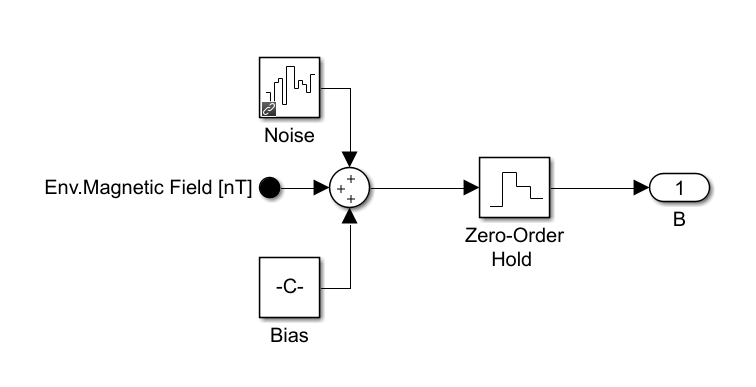
\includegraphics[width=1\textwidth]{2-toolbox/magnetometer.png}
            \caption{SCARS Magnetometer model}
            \label{fig:magnetometer}
        \end{figure}

        To make use of implemented Magnetic Field Model, a model of a set of magnetometers is available as a part of \ac{scars} Toolbox. From magnetometer sensors the measurements of direction and magnitude of magnetic field can be acquired. After comparison with Earth's magnetic model spacecraft's on board software conducts transformation from measured vector to one of the reference frames used by \ac{adcs} subsystem, providing information about its attitude. Due to their light weight, low power consumption and have wide margin for operating temperature, they are a relative sensors to be included on board of a small spacecraft.

        The input for this block is magnetic field strength and the output is measured signal, both in $nT$ unit.
        %cite: MAGNETOMETERS - richard2008 (maybe)

        % \dots\textit{description of implementation}\dots

    \subsubsection{Gyroscopes}
        % https://www.youtube.com/watch?v=anMzEbbbrp8
        % Parameters:
        % \begin{itemize}
        %     \item change over temperature
        %     \item zero rate level change over temperature [dps/*C] (but this can biased to get rid of the error, so is not necessary to model)
        %     \item sensitivity
        %     \item Measurement range
        %     \item Angle Random Walk (same Parameter as FFT and Power Spectral Density)
        % \end{itemize}

        \begin{figure}[H]
            \centering
            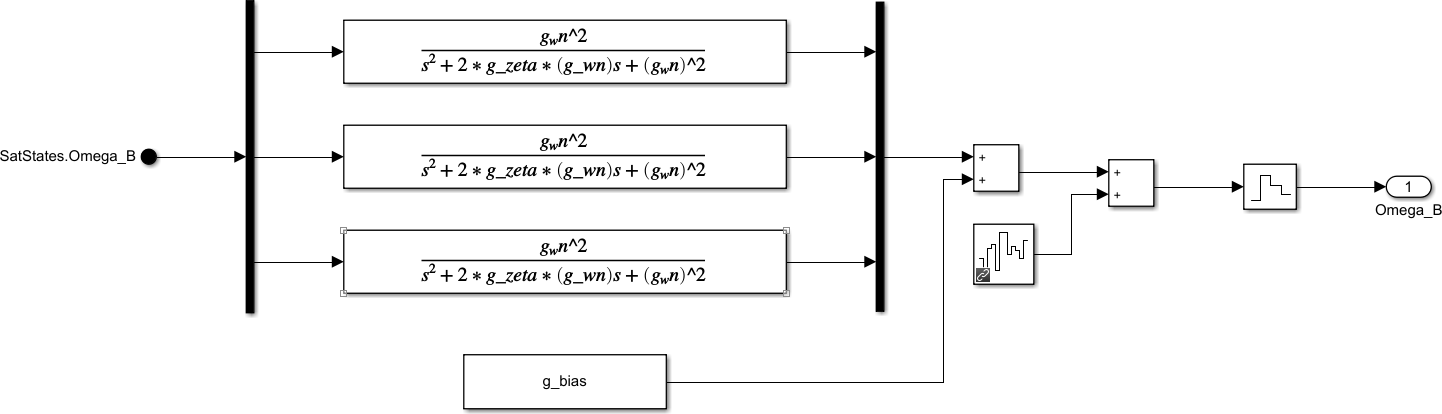
\includegraphics[width=1\textwidth]{2-toolbox/gyroscope.png}
            \caption{SCARS Gyroscope model}
            \label{fig:gryo_simulink}
        \end{figure}

        Gyroscopes, which fall under category of inertial sensors, measure angular rate around fixed axis. In smaller spacecraft, which is in great deal of \ac{scars} toolbox use-cases, the conventional spinning mass gyroscopes are rarely used, due to limitations in mass and size. Recent developments allow for use of much smaller and cheaper \ac{mems} gyroscopes, which are vibrating angular rate sensors. They were chosen to model for the toolbox, as of popularity in projects with highly restricted budget. \cite{armenise2010advances} Inside of vibrating gyroscope the Coriolis effect is a cause the vibrating core to produce a force acting on its support. The measurement of the force is used to determine the rate of rotation of the body around gyroscope axis. \ac{mems} gyros are similar to integrated circuits, which use the miniaturized version of mechanisms based on principles of operation of either vibrating wheels, tuning forks, resonant solids or similar common designs. \cite{bernstein2003overview} While, besides previously mentioned qualities, the upsides of \ac{mems} gyroscopes are availability of both analog and digital outputs, low power consumption and commercial availability. On the other hand, \ac{mems} gyros have shorter lifetime and lower performance when compare to pricier alternatives.

        % In the toolbox the following sources of gyroscope errors are modeled:
        % \begin{itemize}
        %     \item Bias offset:
        %     \item Scale factor: 
        %     \item \ac{arw}: A high frequency noise term that has a correlation time much shorter than the sample time. Can be defined as white noise component on the sensor output. Specified either in $\frac{deg}{\sqrt{h}}$ or, as a power spectral density, in $\frac{(deg/h)^2}{Hz}$. % cite this here: http://citeseerx.ist.psu.edu/viewdoc/download?doi=10.1.1.210.1133&rep=rep1&type=pdf
        %     \item Quantization Error: An error which is caused by the digital quantization of output signal, obtained when sampling analog input.
        %     \item ...
        % \end{itemize}
        
        % write something about second order dynamics

        In \ac{scars} the gyroscope model, as seen on \autoref{fig:gryo_simulink}, includes a second order transfer function, describing the system using parameters such as natural frequency, bandwidth, damping ratio, but also it includes gyroscopic bias and noise source, in attempt to transfer ideal gyroscope into real sensor. 

        % \dots\textit{work in progress}\dots

    %    - Cite this: \cite{kapeelmodeling} % for errors

    % \subsubsection{Inertial Measurement Units}

    \subsubsection{Star Tracker}
        % https://www.youtube.com/watch?v=anMzEbbbrp8
        % Parameters:
        % \begin{itemize}
        %     \item change over temperature
        %     \item zero rate level change over temperature [dps/*C] (but this can biased to get rid of the error, so is not necessary to model)
        %     \item sensitivity
        %     \item Measurement range
        %     \item Angle Random Walk (same Parameter as FFT and Power Spectral Density)
        % \end{itemize}

        \begin{figure}[H]
            \centering
            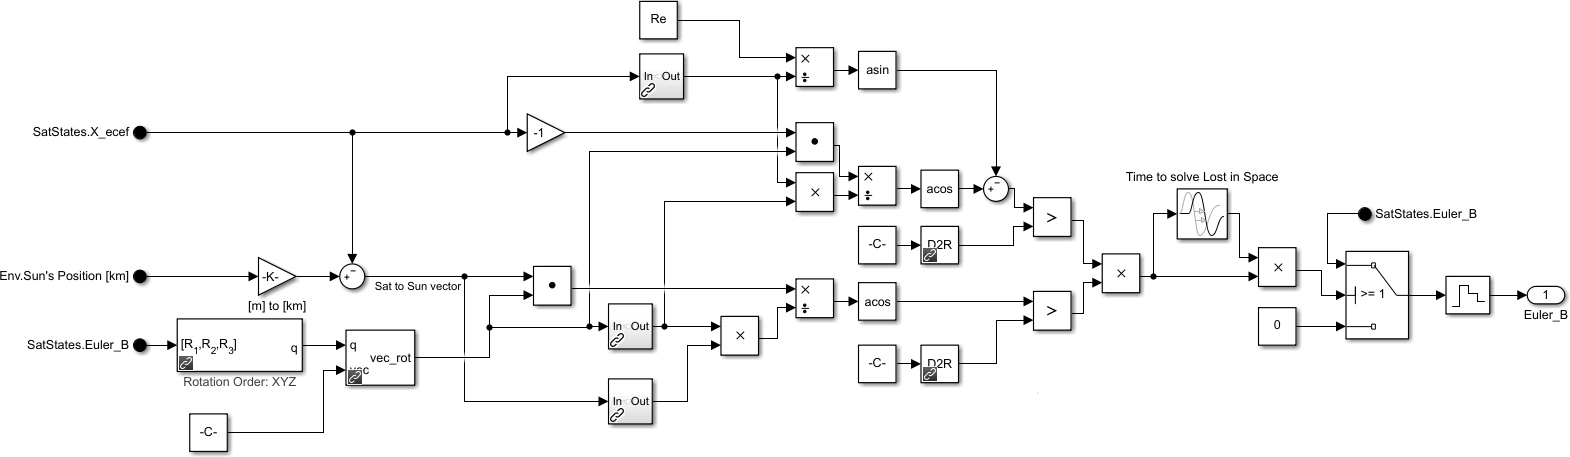
\includegraphics[width=1\textwidth]{2-toolbox/star_tracker.png}
            \caption{SCARS Star Tracker model}
            \label{fig:star_tracker}
        \end{figure}

        A star tracker is an complex attitude sensor, providing the most accurate determination within available commercial solutions. It consist of optical camera and wide array of processing algorithms, which allow to read the position of the stars from captured image and to compare that positions to database of known and visible stars to find the attitude of the spacecraft. Moreover, it can do so without a-priori knowledge, using lost-in-space algorithm\cite{delabie2016star}.

        As simulating stars position to achieve high fidelity star tracker model and using parameters such as camera resolution and algorithm accuracy and precision, it was decided to assume ideal output from star tracker and to focus on mechanical problems, such as blinding the sensitive camera sensor by light from the Sun or reflected by the Earth. As it can be seen on \autoref{fig:star_tracker}, the model calculates the relative position of Sun and satellite, then Earth and satellite and based on this, and two key parameters input by the user - Sun and Earth exclusive angle, provides the actual output or null value, if the star tracker is blinded. Additionally, if the parameter is non-zero given, the model adds the delay of time it takes the software to solve the lost-in-space problem to the null value output duration.
